%%%%%%%%%%%%%%%%%%%%%%%%%%%%%%%%%%%%%%%%%%%%%%%%%%%%%%%%%%%%%%%%%%%%%
%
%  This is a sample LaTeX input file for your contribution to 
%  the M&C2023 topical meeting.
%
%  Please use it as a template for your full paper 
%    Accompanying/related file(s) include: 
%       1. Document class/format file: mc2023.cls
%       2. Sample PDF/Postscript Figure: figure.pdf,figure.ps
%       3. A PDF file showing the desired appearance: mc2023_template.pdf
%       4. cites.sty and citesort.sty that might be needed by some users 
%    Direct questions about these files to: buijsa@mcmaster.ca
%    Originals provided by brantley1@llnl.gov
%
%    Notes: 
%      (1) You can use the "dvips" utility to convert .dvi 
%          files to PostScript.  Then, use either Acrobat 
%          Distiller or "ps2pdf" to convert to PDF format. 
%      (2) Different versions of LaTeX have been observed to 
%          shift the page down, causing improper margins.
%          If this occurs, adjust the "topmargin" value in the
%          mc2023.cls file to achieve the proper margins. 
%
%%%%%%%%%%%%%%%%%%%%%%%%%%%%%%%%%%%%%%%%%%%%%%%%%%%%%%%%%%%%%%%%%%%%%


%%%%%%%%%%%%%%%%%%%%%%%%%%%%%%%%%%%%%%%%%%%%%%%%%%%%%%%%%%%%%%%%%%%%%
\documentclass[letterpaper]{mc2023}
%
%  various packages that you may wish to activate for usage 
\usepackage{tabls}
\usepackage{cites}
\usepackage{epsf}
\usepackage{appendix}
\usepackage{ragged2e}
\usepackage[top=1in, bottom=1in, left=1in, right=1in]{geometry}
\usepackage{enumitem}
\setlist[itemize]{leftmargin=*}
\usepackage{caption}
\captionsetup{width=1.0\textwidth,font={bf,normalsize},skip=0.3cm,within=none,justification=centering}

%\usepackage[justification=centering]{caption}
\usepackage[acronym,toc]{glossaries}

\usepackage{xspace}
\usepackage{tabulary}
\usepackage{subfig}

\newcommand{\Cycamore}{\textsc{Cycamore}\xspace}
\newcommand{\Cyclus}{\textsc{Cyclus}\xspace}
\newcommand{\SaltProc}{\textsc{SaltProc}\xspace}
\newcommand{\OpenMC}{\textsc{OpenMC}\xspace}
\newcommand{\SerpentTWO}{\textsc{Serpent2}\xspace}
\newcommand{\ONIX}{\textsc{ONIX}\xspace}
\newcommand{\NJOYTWOONE}{\textsc{NJOY21}\xspace}
\newcommand{\ChemTriton}{\textsc{ChemTriton}\xspace}
\newcommand{\Shift}{\textsc{Shift}\xspace}
\newcommand{\SCALE}{\textsc{SCALE}\xspace}
\newcommand{\TRITON}{\textsc{TRITON}\xspace}
\newcommand{\ORIGEN}{\textsc{ORIGEN}\xspace}
\newcommand{\MCNPSIX}{\textsc{MCNP6}\xspace}
\newcommand{\CINDERNINETY}{\textsc{CINDER90}\xspace}
\newcommand{\ADDER}{\textsc{ADDER}\xspace}


%
% Define title...
%
\title{Implementation and Validation of OpenMC \\
in a Salt Reprocessing Simulator for Molten Salt Reactors}
%
% ...and authors
%
\author{%
  % FIRST AUTHORS 
  %
  \textbf{O.~Yardas$^1$}\vspace{3pt} \\
  $^1$University of Illinois Urbana-Champaign 1  \\
  Corresponding Address \vspace{6pt}\\ 
  \url{oyardas2@illinois.edu}
}
%
% Insert authors' names and short version of title in lines below
%
\newcommand{\authorHead}{O. Yardas}
\newcommand{\shortTitle}{OpenMC salt reprocessing simulator}
%
%%%%%%%%%%%%%%%%%%%%%%%%%%%%%%%%%%%%%%%%%%%%%%%%%%%%%%%%%%%%%%%%%%%%%
%
%   BEGIN DOCUMENT
%
%%%%%%%%%%%%%%%%%%%%%%%%%%%%%%%%%%%%%%%%%%%%%%%%%%%%%%%%%%%%%%%%%%%%%
\begin{document}
\newacronym{crpg}{CRPG}{Computational Reactor Physics Group}
\newacronym{ornl}{ORNL}{Oak Ridge National Laboratory}
\newacronym{mit}{MIT}{Massachusets Institute of Technology}
\newacronym{csg}{CSG}{constructive solid geometry}
\newacronym{cfd}{CFD}{computational fluid dynamics}
\newacronym{cad}{CAD}{computer aided design}
\newacronym{dnp}{DNP}{delayed neutron precursor}
\newacronym{ghg}{GHG}{greenhouse gas}
\newacronym{gif}{GIF}{Generation IV Interational Forum}
\newacronym{msr}{MSR}{molten salt reactor}
\newacronym{msre}{MSRE}{Molten Salt Reactor Experiment}
\newacronym{msbr}{MSBR}{Molten Salt Breeder Reactor}
\newacronym{msfr}{MSFR}{Molten Sodium Fast Reactor}
\newacronym{nrc}{NRC}{Nuclear Regulatory Commission}
\newacronym{rnd}{R\&D}{research and development}
\newacronym{mns}{M\&S}{modelling and simulation}
\newacronym{ent}{E\&T}{education and training}
\newacronym{doene}{DOE-NE}{Department of Energy Office of Nuclear Energy}
\newacronym{cc}{CC}{closed code}
\newacronym{oss}{OSS}{open source software}
\newacronym{iaea}{IAEA}{International Atomic Energy Agency}
\newacronym{oncore}{ONCORE}{Open-source Nuclear COdes for REactor analysis}
\newacronym{snf}{SNF}{spent nuclear fuel}
\newacronym{doe}{DOE}{Department of Energy}

\maketitle
\justify 
\parskip 6pt plus 1 pt minus 1 pt

\begin{abstract}
%  Anthropogenic \Gls{ghg} emissions drive global warming. Rapid decrease in
%  global \Gls{ghg} emissions can can dampen the impact of global warming.
%  Transitioning to electricity production methods that have no \Gls{ghg}
%  emissions would contribute significantly to global \Gls{ghg} emission
%  reduction.
  Like their contemporary counterparts, next generation nuclear
  reactors will produce no \Gls{ghg} emissions, while being safer and more
  efficient. \Gls{msr} technology is of particular interest due to the
  opportunities and challenges it presents. No operating \Gls{msr}s exist, so we
  must rely on computer simulations to study this technology. Popular \Gls{msr}
  designs to use in simulations include the \Gls{msbr}, the \Gls{msre}, and the
  \Gls{msfr}. A key process to consider for \Gls{msr}s is on-line fuel
  reprocessing and its effect on reactor dynamics. SaltProc is an open source
  interface code tool that simulates on-line fuel reprocessing when coupled with
  a depletion-capable transport solver. SaltProc was intended to be usable with
  any depletion solver, but only had support for Serpent2. I overhauled the
  SaltProc code to simplify coupling supports for depletion solvers, and added
  support for OpenMC. I also validated the new functionality on a full-core model
  of the \Gls{msbr}. This is significant as this makes SaltProc the first
  completely open-source tool to simulate on-line fuel reprocessing.
\end{abstract}
\vspace{6pt}
\keywords{MSR, reprocessing, OpenMC}

\section{INTRODUCTION} 
%Nuclear power currently constitutes one fifth of US domestic electricity
%production and half of US zero-carbon electricity production
%\cite{eia_faq_2021} \cite{doene_facts_2021}. Unfortunately, our current nuclear
%fleet faces several threats to its long-term survival, the most relevant being
%the state of the electricity market: record-low natural gas prices and
%increases in subsidies for renewables without similar compensation for
%nuclear make it uncompetitive in the current market and economically unsustainable in the
%long term if current conditions continue\footnote{This is a generalization as
%the economics of electricity markets is incredibly complex and requires more space that I can give to it
%in this abstract to fully appreciate} \cite{szilard_economic_2016}.
%%perhaps mention all plants that have been shut down recently?

%Assuming that we resolve the economic threats to our current nuclear fleet,
%at some point in the future, we will need to shut down and decommission them.
%To maintain nuclear power's position in our decarbonization technology stack, we
%will need to develop and implement new kinds of nuclear reactors that are more
%sustainable, economically competitive, safe, and reliable than their
%predecessors.
%% I want to make this point differently... the conclusion should be that we need new nuclear power tech to ensure we can decarbonize, but I don't feel like the preceding statements smoothly come to that conclusion in the way I have preseneted them here
 
%\subsection{Molten Salt Reactors}%
%\label{sec:molten_salt_reactors}
The next generation of nuclear power reactors will need to rapidly respond to
increasing electricity consumption and the need for decarbonization. These
reactiors need to be built quickly and have widespread use, while maintaining or
increasing fuel efficiency, economic competitiveness, safety, and proliferation
resistance.

This is the conclusion that the \Gls{gif} came to in their 2002
roadmap \cite{doe-ne_technology_2002}. \Gls{gif} selected six reactor
technologies in total. One of them, the \Gls{msr},\footnote{for
this paper {\it Molten Salt Reactor} refers specifically to the reactor type
where the fissile material is dissolved in in the salt coolant} is of
particular interest due to the unique challenges and opportunities it presents
for new nuclear fuel cycles, proliferation safeguards, and multiphysics
modeling.
%% why the msr??

The \Gls{msr} uses a mixture of liquid-phase salts as a coolant and solvent for
the fuel. Liquid fuel enables the adoption of {\it online reprocessing} by
pumping used fuel out of the reactor and pumping fresh or reprocessed fuel back
into the reactor.\footnote{this concept is known as {\it separations and feeds}}
This enables the removal of undesirable fission products produced by the fission
reaction. In contrast, the fission
products remain trapped in solid fuel used in contemporary rectors, which can
reduce the thermal performance of the fuel via thermal cracking as well as
absorb neutrons that would otherwise contribute to the fission reaction. 

%\Gls{msr}s face several technical and logistical challenges before we can
%deploy them for civilian power generation. High temperature liquid-phase salt
%will steadily corrode metals over time, so the reactor vessel of a \Gls{msr}
%must use special corrosion-resistant materials. High temperature salt itself is
%extremely hazardous and reacts explosively with moisture, so workers handling
%fuel salt must use special procedures and PPE. Remote handling of fuel salt may
%be necessary in some or all instances. Even with such challenges, I believe the
%potential benefits of \Gls{msr} technology merit its development.

\Gls{mns} codes will play a critical role in licensing GenIV reactors. In
preparation for \Gls{msr}s, both the \Gls{doene} and the \Gls{nrc}
identified several technical gaps in current \Gls{mns} tools that are necessary
for efficient and effective license application reviews
\cite{betzler_modeling_2019} \cite{usnrc_nonlwr_2020-1}. In particular, both the
\Gls{doene} and the \Gls{nrc} have identified fuel composition and its
evolution in a \Gls{msr} to be key modeling features necessary for accident
analysis. 

\subsection{\Gls{msr} Depletion Codes}%
\label{sec:msr_codes}

To model the changing fuel composition in a \Gls{msr}, there are at least two
processes we must consider:
\begin{enumerate}
    \item Fuel {\it depletion}\footnote{the consumption of fissile material in the fuel and production of fission products via the fission chain reaction}
    \item Removal and feed processes
\end{enumerate}

We can concisely describte the rate of change of the number density of $n$ nuclides with the equation:
\begin{align}
    \label{eq:bateman-1}
    \frac{d}{dt}N(t) = \mathbf{A}N(t)
\end{align}

where $N$ is a $n$-vector and $\mathbf{A}$ is the depletion matrix\footnote{this
matrix contains all the coefficient terms in the Bateman equation}.
Incorporating removals and feeds into equation \ref{eq:bateman-1} involves
the addition of a time dependent removal factor $r_{i}(t)$ and feed factor
$f_{i}(t)$ for each nuclide $i$, which in matrix form we express as:
\begin{align}
    \label{eq:bateman-1}
    \frac{d}{dt}N(t) = \mathbf{A}N(t) + S(t)
\end{align}

where $S$ is an $n$-vector containing the sums of the removal and feed terms
for each nuclide $i$. This equation describes {\it continuous reprocessing}.
The additional term in equation from continuous reprocessing increases
computational cost and implementation difficulty and may require a different set
of preconditioners for numerical stability and convergence.

Alternatively, one could run a depletion simulation, perform the removals and
feeds in an external application on the resulting material composition, and run
another depletion simulation on the reprocessed composition. This procedure
models {\it batch-wise reprocessing}, in which material from the core is
reprocessed at regular intervals rather than continuously. Batch-wise
reprocessing enables flexibility in the choice of depletion solver, as an
external software tool can perform the reprocessing step and feed the results
back into the depletion solver.

\begin{table}[htpb]
    \centering
    \caption{Software tools that can model \Gls{msr} depletion with fuel reprocessing}
    \label{tab:msr_depletion_tools}
    \begin{tabulary}{\linewidth}{|C|C|C|C|}
        \hline
        Software tool & Description & Reprocessing scheme & Citation\\
        \hline
        \ADDER & Interface code with internal depletion capabilities & Component-based continuous & \cite{nelson_molten_2021}\\
        \hline
        \SCALE & Suite code & Continuous & \cite{betzler_molten_2019}\\
        \hline
        \SerpentTWO & Depletion code & Continuous & \cite{aufiero_extended_2013}\\
        \hline
        \SaltProc & Interface code & Component-based batch-wise & \cite{rykhlevskii_saltproc_2018}\\
        \hline
    \end{tabulary}
\end{table}


\SaltProc\cite{rykhlevskii_saltproc_2018}, the subject of this paper, is an open
source tool for simulating reactor physics in \Gls{msr}s that uses a batch-wise
reprocessing approach to model the fuel composition evolution. \SaltProc uses
\SerpentTWO\cite{leppanen_serpent_2014} to run depletion simulations.
While other software with comparable capabilities exist (see Table
\ref{tab:msr_depletion_tools}), \SaltProc is uniqe among its peers as an open
source project.

%Historically, software used in licensing, \gls{rnd}, and \gls{ent} efforts in
%the nuclear field have been closed source and proprietary. For \Gls{rnd} and
%\Gls{ent} efforts in particular, the liscening process can bring collaborative
%efforts to a grinding halt. Using \gls{cc}s in scientific publications and
%research presents barriers to reproducibility and the ability of external
%verification of results.
    
%Regulatory bodies will require new software features (and, in some cases, entirely
%new software tools) to effectively and efficiently perform licensing
%activities for the next generation of advanced reactor designs
%\cite{usnrc_nonlwr_2020-1}, and many of the open source tools emerging in the
%past decade (e.g., \OpenMC\cite{romano_openmc_2015}) have the advantage over
%their legacy \Gls{cc} ancestors (e.g., \SerpentTWO \cite{leppanen_serpent_2014})
%of using best-practices for software development. Thus, the features
%and tools required may be more readily implementable and usable in open source projects than
%in closed codes.

%We are entering the era of \gls{oss} purpose-built for nuclear
%science and engineering applications. The number of open source projects in this
%field
%(\ONIX\cite{de_troullioud_de_lanversin_onix_2021}, \OpenMC,
%\NJOYTWOONE\cite{noauthor_njoy21_2022}, \Cyclus\cite{noauthor_cyclus_2022}, to
%name a few) is growing in recognition of the need for distributable,
%high-quality, and transparent software tools. The \Gls{iaea} facilitated
%\Gls{oncore} initiative \cite{fiorina_initiative_2021} is the best
%example of the push towards \Gls{oss}, as seen in the mission statement: to
%``[promote] development and application of open-source multi-physics simulation
%tools to support research, education, and training for analysis of advanced
%nuclear power reactors'' \cite{iaea_open-source_2022}. 

I am working on implenting support for \OpenMC's depletion solver in SaltProc,
and will verify my implementation on a model of the MSBR.

\section{MOLTEN SALT REACTOR MODEL}
\label{sec:msr-model}

The \OpenMC \Gls{msbr} model is a reproduction of the on the \SerpentTWO \Gls{msbr} model in \cite{rykhlevskii_modeling_2019}, which in turn is based on
the specifications of the MSBR design report \cite{robertson_conceptual_1971}.
The MSBR geometry is extremely complicated, and as such the model presented here
is a simplified version from the one in the paper. These differences can be seen in Figures \ref{fig:msbr_openmc_model} and \ref{fig:msbr_original_detail}.

\begin{figure}[htpb]
    \centering
    \subfloat[][]{
        
\includegraphics[width=0.25\linewidth]{figs/msbr_model_section.png}
        \label{fig:msbr_openmc_model}
    }
    \subfloat[][]{
        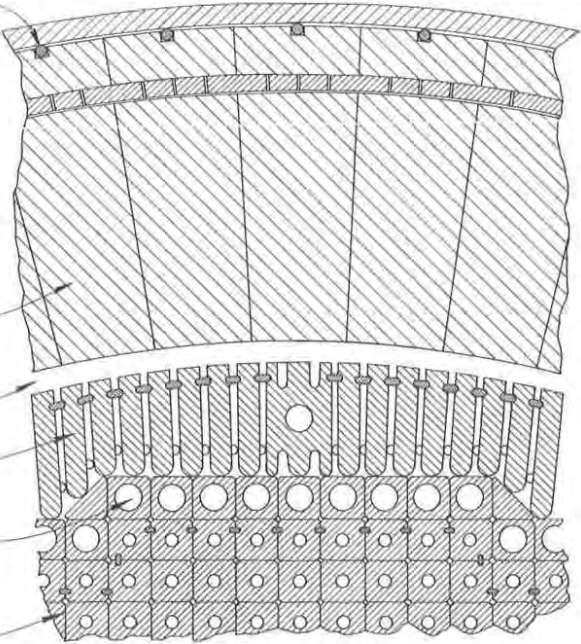
\includegraphics[width=0.25\linewidth]{figs/msbr_original_section.png}
        \label{fig:msbr_original_detail}
    }
    \caption[\Gls{msbr} model comparison]{\subref{fig:msbr_openmc_model} Detail
    of the OpenMC \Gls{msbr} model; \subref{fig:msbr_original_detail} Detail of
    the \Gls{msbr} design in the original paper}
\end{figure}


\section{CURRENT AND ONGOING WORK}

The \OpenMC MSBR model has been verified against the \SerpentTWO model in both
a neutron transport simulation, and a depletion simulation.

I currently working on finishing implementation of \OpenMC support in \SaltProc
so I can test the model in the intended application.

%\section*{NOMENCLATURE}
%
%If variables are extensively used in the text, a Nomenclature section would be helpful to the readers.

\section*{ACKNOWLEDGEMENTS}
I would like to acklowledge Dr. Madicken Munk for her review of this manuscript.
This work was funded by the NRC Integrated University Grant Program Fellowship.

% You can enter a bibliography into the document using either BibTex with the bibliography
% style file "mc2023.bst" found in the template directory or using the standard LaTeX
% thebibliography environment.
\newif\ifusebibtex
%\usebibtexfalse
\usebibtextrue

\ifusebibtex
\setlength{\baselineskip}{12pt}
\bibliographystyle{mc2023}
\bibliography{mc2023}
\else
\setlength{\baselineskip}{12pt}
\begin{thebibliography}{300}
\bibitem{journal} B. Author(s), ``Title, using capitalization'' \emph{Journal Name in Italic}, 
  \textbf{Volume in Bold}, pp. 34-89 (20xx).
\bibitem{proc_paper} C. D. Author(s), ``Article Title,'' \emph{Proceedings of
  Meeting in Italic}, Location, Dates of Meeting, Vol. n, pp. 134-156 
  (20xx).
\bibitem{book} E. F. Author, \emph{Book Title in Italic}, Publisher, City \&
  Country (20xx). 
\bibitem{website} ``Canadian SMR Roadmap,'' \\
  \url{https://smrroadmap.ca/wp-content/uploads/2018/12/Technology-WG.pdf} (2018).
\end{thebibliography}
\fi

%\appendix
%\gdef\thesection{APPENDIX~\Alph{section}}
%\section{Sample Appendix 1}
%\label{app:a}
%If necessary, include Appendices numbered in upper case alphabetical order. This is \ref{app:a}. 



\end{document}
